\documentclass[]{article}
\usepackage{lmodern}
\usepackage{amssymb,amsmath}
\usepackage{ifxetex,ifluatex}
\usepackage{fixltx2e} % provides \textsubscript
\ifnum 0\ifxetex 1\fi\ifluatex 1\fi=0 % if pdftex
  \usepackage[T1]{fontenc}
  \usepackage[utf8]{inputenc}
\else % if luatex or xelatex
  \ifxetex
    \usepackage{mathspec}
    \usepackage{xltxtra,xunicode}
  \else
    \usepackage{fontspec}
  \fi
  \defaultfontfeatures{Mapping=tex-text,Scale=MatchLowercase}
  \newcommand{\euro}{€}
\fi
% use upquote if available, for straight quotes in verbatim environments
\IfFileExists{upquote.sty}{\usepackage{upquote}}{}
% use microtype if available
\IfFileExists{microtype.sty}{%
\usepackage{microtype}
\UseMicrotypeSet[protrusion]{basicmath} % disable protrusion for tt fonts
}{}
\usepackage[margin=1in]{geometry}
\usepackage{color}
\usepackage{fancyvrb}
\newcommand{\VerbBar}{|}
\newcommand{\VERB}{\Verb[commandchars=\\\{\}]}
\DefineVerbatimEnvironment{Highlighting}{Verbatim}{commandchars=\\\{\}}
% Add ',fontsize=\small' for more characters per line
\usepackage{framed}
\definecolor{shadecolor}{RGB}{248,248,248}
\newenvironment{Shaded}{\begin{snugshade}}{\end{snugshade}}
\newcommand{\KeywordTok}[1]{\textcolor[rgb]{0.13,0.29,0.53}{\textbf{{#1}}}}
\newcommand{\DataTypeTok}[1]{\textcolor[rgb]{0.13,0.29,0.53}{{#1}}}
\newcommand{\DecValTok}[1]{\textcolor[rgb]{0.00,0.00,0.81}{{#1}}}
\newcommand{\BaseNTok}[1]{\textcolor[rgb]{0.00,0.00,0.81}{{#1}}}
\newcommand{\FloatTok}[1]{\textcolor[rgb]{0.00,0.00,0.81}{{#1}}}
\newcommand{\CharTok}[1]{\textcolor[rgb]{0.31,0.60,0.02}{{#1}}}
\newcommand{\StringTok}[1]{\textcolor[rgb]{0.31,0.60,0.02}{{#1}}}
\newcommand{\CommentTok}[1]{\textcolor[rgb]{0.56,0.35,0.01}{\textit{{#1}}}}
\newcommand{\OtherTok}[1]{\textcolor[rgb]{0.56,0.35,0.01}{{#1}}}
\newcommand{\AlertTok}[1]{\textcolor[rgb]{0.94,0.16,0.16}{{#1}}}
\newcommand{\FunctionTok}[1]{\textcolor[rgb]{0.00,0.00,0.00}{{#1}}}
\newcommand{\RegionMarkerTok}[1]{{#1}}
\newcommand{\ErrorTok}[1]{\textbf{{#1}}}
\newcommand{\NormalTok}[1]{{#1}}
\usepackage{graphicx}
\makeatletter
\def\maxwidth{\ifdim\Gin@nat@width>\linewidth\linewidth\else\Gin@nat@width\fi}
\def\maxheight{\ifdim\Gin@nat@height>\textheight\textheight\else\Gin@nat@height\fi}
\makeatother
% Scale images if necessary, so that they will not overflow the page
% margins by default, and it is still possible to overwrite the defaults
% using explicit options in \includegraphics[width, height, ...]{}
\setkeys{Gin}{width=\maxwidth,height=\maxheight,keepaspectratio}
\ifxetex
  \usepackage[setpagesize=false, % page size defined by xetex
              unicode=false, % unicode breaks when used with xetex
              xetex]{hyperref}
\else
  \usepackage[unicode=true]{hyperref}
\fi
\hypersetup{breaklinks=true,
            bookmarks=true,
            pdfauthor={Martin Cote},
            pdftitle={Exponential Distribution Investigation in R - Statistical Inference: Course Project - Question 2},
            colorlinks=true,
            citecolor=blue,
            urlcolor=blue,
            linkcolor=magenta,
            pdfborder={0 0 0}}
\urlstyle{same}  % don't use monospace font for urls
\setlength{\parindent}{0pt}
\setlength{\parskip}{6pt plus 2pt minus 1pt}
\setlength{\emergencystretch}{3em}  % prevent overfull lines
\setcounter{secnumdepth}{0}

%%% Use protect on footnotes to avoid problems with footnotes in titles
\let\rmarkdownfootnote\footnote%
\def\footnote{\protect\rmarkdownfootnote}

%%% Change title format to be more compact
\usepackage{titling}
\setlength{\droptitle}{-2em}
  \title{Exponential Distribution Investigation in R - Statistical Inference:
Course Project - Question 2}
  \pretitle{\vspace{\droptitle}\centering\huge}
  \posttitle{\par}
  \author{Martin Cote}
  \preauthor{\centering\large\emph}
  \postauthor{\par}
  \predate{\centering\large\emph}
  \postdate{\par}
  \date{April 26, 2015}


\usepackage{graphicx}


\begin{document}

\maketitle


\section{Overview}\label{overview}

Analysis of the ToothGrowth data from the R datasets package, as part of
the Statistical Inference course from Coursera.

\section{Required tools}\label{required-tools}

Loading the required libraries.

\begin{verbatim}
## 
## Attaching package: 'dplyr'
## 
## The following object is masked from 'package:stats':
## 
##     filter
## 
## The following objects are masked from 'package:base':
## 
##     intersect, setdiff, setequal, union
\end{verbatim}

\section{Exploratory Data Analysis}\label{exploratory-data-analysis}

\subsection{Overall analysis, by dose and
supplement}\label{overall-analysis-by-dose-and-supplement}

\begin{Shaded}
\begin{Highlighting}[]
\CommentTok{# Load the data and convert to DPLYR data.frame}
\KeywordTok{attach}\NormalTok{(ToothGrowth)}
\NormalTok{data <-}\StringTok{ }\KeywordTok{tbl_df}\NormalTok{(ToothGrowth)}

\CommentTok{# Plot the length changes by the dose and type of supplement}
\KeywordTok{ggplot}\NormalTok{(data, }\KeywordTok{aes}\NormalTok{(dose, len)) +}
\StringTok{  }\KeywordTok{geom_point}\NormalTok{(}\KeywordTok{aes}\NormalTok{(}\DataTypeTok{color =} \NormalTok{supp), }\DataTypeTok{size=}\DecValTok{4}\NormalTok{, }\DataTypeTok{alpha=}\DecValTok{1}\NormalTok{/}\DecValTok{2}\NormalTok{) +}
\StringTok{  }\KeywordTok{xlab}\NormalTok{(}\StringTok{"Dose"}\NormalTok{) +}
\StringTok{  }\KeywordTok{ylab}\NormalTok{(}\StringTok{"Tooth Length"}\NormalTok{) +}
\StringTok{  }\KeywordTok{labs}\NormalTok{(}\DataTypeTok{title=}\StringTok{"ToothGrowth Exploratory Analysis (divide by Supplement Type)"}\NormalTok{) +}
\StringTok{  }\KeywordTok{theme_bw}\NormalTok{()}
\end{Highlighting}
\end{Shaded}

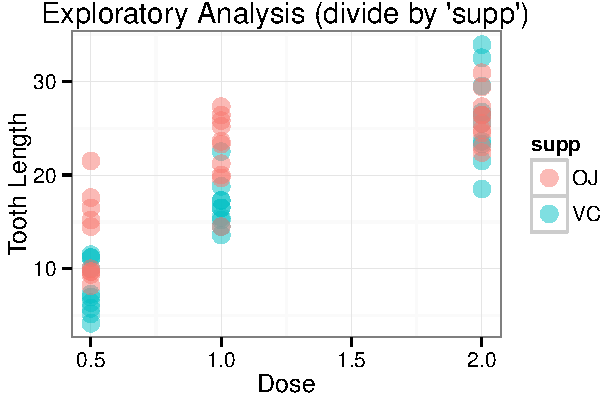
\includegraphics{statinference-courseproject-1-Question-2_files/figure-latex/unnamed-chunk-2-1.pdf}

From the plot above, it seems the `supp' (Supplement Type) doesn't
impact the tooth growth although as the dosage increases, there seems to
be a clear increase in tooth growth.

\subsection{Analysis, by dose only}\label{analysis-by-dose-only}

\begin{Shaded}
\begin{Highlighting}[]
\CommentTok{# Summarise the data by dose and average changes of teeth}
\NormalTok{data_bydose <-}\StringTok{ }\NormalTok{data %>%}
\StringTok{  }\KeywordTok{group_by}\NormalTok{(dose) %>%}
\StringTok{  }\KeywordTok{summarise}\NormalTok{(}\DataTypeTok{AVG =} \KeywordTok{mean}\NormalTok{(len))}

\CommentTok{# Plot the length changes by the dose only}
\KeywordTok{ggplot}\NormalTok{(data_bydose, }\KeywordTok{aes}\NormalTok{(dose, AVG)) +}
\StringTok{  }\KeywordTok{geom_line}\NormalTok{(}\DataTypeTok{color=}\StringTok{"steelblue"}\NormalTok{, }\DataTypeTok{size=}\DecValTok{2}\NormalTok{, }\DataTypeTok{alpha=}\DecValTok{1}\NormalTok{/}\DecValTok{2}\NormalTok{) +}
\StringTok{  }\KeywordTok{xlab}\NormalTok{(}\StringTok{"Dose"}\NormalTok{) +}
\StringTok{  }\KeywordTok{ylab}\NormalTok{(}\StringTok{"Tooth Length"}\NormalTok{) +}
\StringTok{  }\KeywordTok{labs}\NormalTok{(}\DataTypeTok{title=}\StringTok{"ToothGrowth Exploratory Analysis"}\NormalTok{) +}
\StringTok{  }\KeywordTok{theme_bw}\NormalTok{()}
\end{Highlighting}
\end{Shaded}

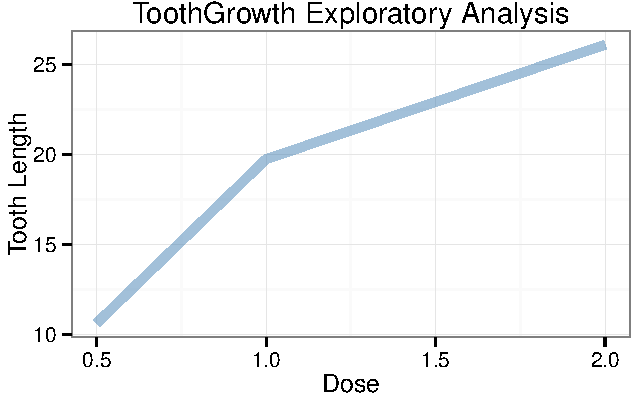
\includegraphics{statinference-courseproject-1-Question-2_files/figure-latex/unnamed-chunk-3-1.pdf}

From the latest plot, it seems clearer that as the dose increases, the
tooth length changes increase.

\subsection{Summary of the data}\label{summary-of-the-data}

\begin{Shaded}
\begin{Highlighting}[]
\CommentTok{# Basic summary of the data}
\KeywordTok{summary}\NormalTok{(data)}
\end{Highlighting}
\end{Shaded}

\begin{verbatim}
##       len        supp         dose      
##  Min.   : 4.20   OJ:30   Min.   :0.500  
##  1st Qu.:13.07   VC:30   1st Qu.:0.500  
##  Median :19.25           Median :1.000  
##  Mean   :18.81           Mean   :1.167  
##  3rd Qu.:25.27           3rd Qu.:2.000  
##  Max.   :33.90           Max.   :2.000
\end{verbatim}

\section{Confidence Intervals and Hypothesis
Tests}\label{confidence-intervals-and-hypothesis-tests}

\subsection{Assumptions}\label{assumptions}

\begin{enumerate}
\def\labelenumi{\arabic{enumi}.}
\itemsep1pt\parskip0pt\parsep0pt
\item
  `len' is a continuous random variable, hence using a T distribution
  (as a better alternative to a normal distribution)
\item
  The observations are unrelated and independent (hence, using the
  ``Independent T Confidence Intervals'')
\end{enumerate}

\subsection{Condidence Intervals}\label{condidence-intervals}

\begin{Shaded}
\begin{Highlighting}[]
\CommentTok{# Testing dose}
\KeywordTok{t.test}\NormalTok{(data$len, data$dose, }\DataTypeTok{paired=}\OtherTok{FALSE}\NormalTok{, }\DataTypeTok{var.equal=}\OtherTok{FALSE}\NormalTok{)}
\end{Highlighting}
\end{Shaded}

\begin{verbatim}
## 
##  Welch Two Sample t-test
## 
## data:  data$len and data$dose
## t = 17.8096, df = 59.798, p-value < 2.2e-16
## alternative hypothesis: true difference in means is not equal to 0
## 95 percent confidence interval:
##  15.66453 19.62881
## sample estimates:
## mean of x mean of y 
## 18.813333  1.166667
\end{verbatim}

\begin{Shaded}
\begin{Highlighting}[]
\CommentTok{# Testing supp}
\KeywordTok{t.test}\NormalTok{(data$len ~}\StringTok{ }\NormalTok{data$supp)}
\end{Highlighting}
\end{Shaded}

\begin{verbatim}
## 
##  Welch Two Sample t-test
## 
## data:  data$len by data$supp
## t = 1.9153, df = 55.309, p-value = 0.06063
## alternative hypothesis: true difference in means is not equal to 0
## 95 percent confidence interval:
##  -0.1710156  7.5710156
## sample estimates:
## mean in group OJ mean in group VC 
##         20.66333         16.96333
\end{verbatim}

\subsection{Conclusions}\label{conclusions}

\begin{enumerate}
\def\labelenumi{\arabic{enumi}.}
\itemsep1pt\parskip0pt\parsep0pt
\item
  Strong relation as the dose increases, the changes to the tooth growth
  increase.
\item
  No relation can be made between the changes in tooth growth and the
  supplement type.
\end{enumerate}

\end{document}
